\documentclass[a4paper]{article}
\usepackage{geometry}
\geometry{left=3.5cm,right=3.5cm,top=3.5cm,bottom=3.5cm}
\usepackage{amsmath, amssymb}
\usepackage{graphicx}
\usepackage{subfigure}
\usepackage{pdfpages}
\usepackage{multirow}

\usepackage{xeCJK}
\setmainfont{Times New Roman}
\setCJKmainfont[BoldFont=SimHei,ItalicFont=KaiTi]{SimSun}

\usepackage{indentfirst}
\setlength{\parindent}{2em}

\usepackage{fancyhdr}
\pagestyle{fancy}
\usepackage{lastpage}
\rhead{}
\lhead{}
\cfoot{\thepage{}}
\renewcommand{\headrulewidth}{0pt}
\renewcommand{\figurename}{图}
\renewcommand{\tablename}{表}
\renewcommand{\abstractname}{摘要}
\renewcommand{\contentsname}{\CJKfamily{SimHei} 目录}

\headheight 14pt

\usepackage{float}

\renewcommand\baselinestretch{1.2}

\begin{document}

%\begin{titlepage}
%\includepdf[pages=2-3,offset=0cm 0cm]{title.pdf}
%\end{titlepage}

\begin{Huge}
	\centering{\textbf{城市表层土壤重金属污染的建模与分析}}
\end{Huge}
\begin{large}
	\begin{flushright}
		
	\end{flushright}
\end{large}
\ \ \\\\

\begin{abstract}
\textit{}
\end{abstract}

\newpage

\tableofcontents

\newpage

\part{引言}
土壤是生态环境的重要组成部分, 也是人类赖以生存的重要自然资源。然而,随着工农业的发展,土壤污染问题越来越突出,尤其是重金属污染,对于土壤的污染尤其严重。
所谓土壤重金属污染是指由于人类的活动将重金属带入土壤中,致使土壤重金属含量明显高于其自然背景值,并造成生态破坏和环境质量恶化的现象。
当前,随着全球经济一体化的发展,我国也加快了工业化与城市化的发展进程,城市的农业集约化程度不断提高。
生产过程中的固体废物不断向土壤表面堆放和倾倒,有害废水不断向土壤中渗透,汽车排放的废气,大气中的有害气体及飘尘不断随雨水降落在土壤中。
这导致水土资源快速恶化和萎缩,土壤利用强度日益加大。   \\
\indent 城市土壤供应着城市绿色植物的生长介质和养分,是城市污染物重要的源和汇,是土壤微生物的栖息地和能量来源,直接影响到城市的生态环境质量。
重金属污染物主要包括汞、镐、铅、铬、锌、铜、镍、钴、锡以及类金属砷等,作为一种持久性有毒物质,进入土壤系统。
从而会使城市土壤的各种性质发生了变化,引起土壤的组成结构和功能发生变化,微生物活动受到抑制,有害物质或分解产物在土壤中逐渐积累,间接被人体吸收,危害人体健康。
因此,土壤重金属污染已成为全球面临的一个严重环境问题。   \\
\indent 国土资源部统计表明,全国320个严重污染区约有548万hm2土壤,大田类农产品污染超标面积占污染区农田面积的20\%,其中重金属污染占80\%,粮食中重金属镉、砷、铬、铅、汞等的超标率占10\%。
在城市,土地污染问题也十分严重。例如,被公认为城市环境质量优良的公园却也存在着严重的土壤重金属污染。
而且我国每年有 1200 万吨粮食遭到重金属污染,直接经济损失超过 200 亿元。
从我国的土地资源情况来看,人均土地资源远远低于世界平均水平,仅及世界人均占有量的1/3。我国耕地人均只有0.1公顷,为世界人均耕地的27.7%。
由此可见,目前我国土地重金属污染非常严重,而且还影响了到人们的食品安全乃至人们的身体健康。
因而如何有效地治理土地重金属污染问题,改良土壤状况,是目前生态环境保护的一个重要主题。    \\
\indent 对于城市而言,土壤的重金属污染治理也十分重要。如果治理不到位,对于城市居民的生命健康会造成巨大的影响。
同时,城市是一个功能极其多样化的地域,粗略地看,城市一般可分为以下 5 类:生活区、工业区、山区、主干道路和公园绿地区,分别记为 1 类区、2 类区、3 类区、4 类区和 5类区。
显然,不同的功能区对于城区而言具有不同的功能,反之,不同的功能区受人类活动影响的程度也不同,重金属的污染程度也不尽相同,治理过程中也应该有所区别。
\indent 现在要求对某一个城区表层的土壤重金属污染进行调查分析。
首先,将所要调查的城区划分成间距为 1 千米的网格状子区域,接着按照每平方公里 1 个采样点的规则,对
表层土壤(大约为 0~10cm 深度)进行采样并编号,然后用 GPS 对采样点定位,记录采样点的位置,包括海拔。
通过专门的仪器测试分析,进一步获得每个样本点所含的多种化学元素的浓度。
此外,还在远离城区和人类活动的地方,按照每两公里 1 个采样点的规则对表层土进行采样,由于人类很少涉足,土壤几乎没有被污染,故可以把其作为城
区表层土壤中化学元素的背景值。\\

\indent 本文以某市不同功能区的表层土壤为研究对象,对土壤中重金属 As、Cd、Cr、
Cu、Hg、Ni、Pb、Zn 的浓度进行测定所获数据进行分析,评价土壤中重金属的污染程度,分析污染的主要原因并定位污染源。
研究过程主要包括以下几个部分:\\
1)给出 8 种主要重金属元素在该城区的空间分布,并分析该城区内不同区域重金属的污染程度。\\
2)通过对数据进行分析,说明造成重金属污染的主要原因。  \\
3)分析重金属污染物的传播特征,并基于此建立数学模型,确定污染源的位置。  \\
4)分析所建立模型的优缺点。为更好地研究城市地质环境的演变模式,确定应该收集的数据信息。基于这些信息,建立一个可以研究地质环境演变模式的模型。  \\

\part{重金属在不同区域的分布情况}
\indent 土壤重金属污染问题成因可能为工业、交通、燃煤、矿区和人类生活等等。在治理过程中,调查清楚某个地区重金属污染的形成原因,对于污染的治理至关重要。
而了解重金属污染的空间分布情况,可以有效的帮助我们判断某个区域污染的缘由。
所以我们首先对重金属的空间分布情况进行研究。这里我们得到了不同重金属的平面分布,海拔分布以及在不同功能区的分布。   \\
\section*{记号表}
\begin{table}[H]
	\centering
	\caption{}
	\label{tab:problem1_symbols}
	\begin{tabular}{ccc}
		\hline
		符号 & 含义  \\
		\hline
		$(x,y,h)$ &取样点的坐标表示   \\
		$C_{ij}$ & 第i个采样点第j种金属的浓度  \\
		$\nu_j$   &  第j种重金属在土壤中含量的平均值  \\
		$\sigma_j$  &   第j种重金属在土壤中含量的标准差 \\
         $\kappa$ & 元素在土壤中的扩散系数      \\
		$\tau$   & 元素在土壤中的对流系数      \\
		$\rho(x,y,h,t)$   & 第j种金属在点(x,y,h)时间t时的浓度 \\	
	\end{tabular} \\
\end{table}

\section{重金属的平面分布}
由所给数据中的采样点的x,y坐标以及对应的重金属浓度,我们做出了相应的平面分布图,如下图\ref{fig:char}显示了As以及Pb的污染情况平面图。其中不同颜色表示不同功能区。
圆圈的半径大小与污染程度成正比,即污染越严重,圆圈就越大。
\begin{figure}[h]
	\begin{minipage}[t]{0.5\linewidth}
    \centering
    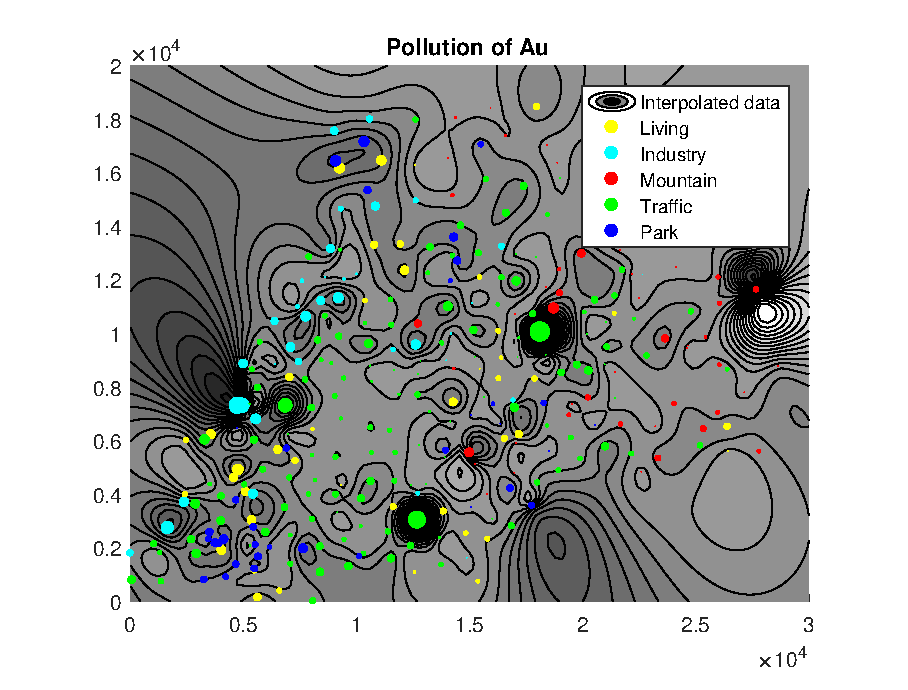
\includegraphics[scale=0.5]{pictures/pollution-of-Au.eps}
    \end{minipage}
    \begin{minipage}[t]{0.5\linewidth}
    \centering 
	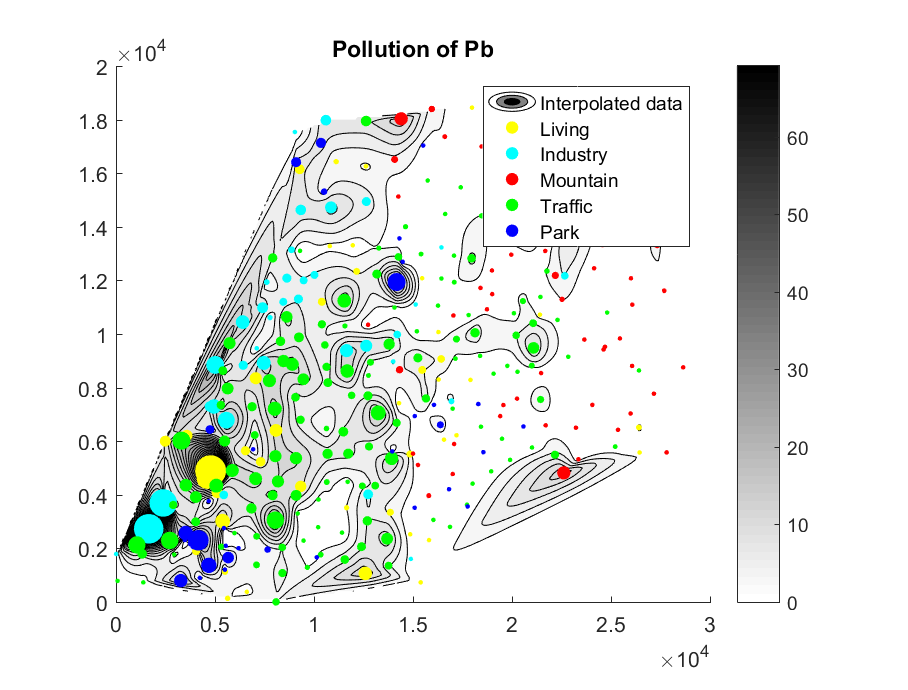
\includegraphics[scale=0.5]{pictures/pollution-of-Pb.eps}
    \end{minipage}
    \label{fig:char}
\end{figure}
从图中能够可以看出:
\indent (1)重金属的分布具有富集性,即重金属在某个区域的分布含量很高,而在其他地方则含量较低。 \\
\indent (2)可以看出As在工业区的分布比较集中,而Pb在交通区域的分布非常密集。                \\
\indent (3)通过对其他重金属元素的平面分布的分析,我们发现不同重金属的分布具有鲜明的特征。往往在某一个区的分布非常密集。 \\
进一步的分析表明:重金属的富集状态实际上是与区域的功能划分息息相关。
比如As主要分布于工业区,这是因为As是一种十分重要化工原料,在工业生产中必不可少,从而在工业区土壤中As含量很高。

\section{重金属的海拔分布}
将海拔每 10 米分一段,假设在某段中共有m个采样点,第i个采样点的重金属j的实测含量为$C_{ij}$,则该段中重金属j的平均含量$W_j$为:
\begin{equation}
W_j=\frac{1}{m}\sum_{i=1}^m C_{ij}
\end{equation}
根据上式,利用采样所得数据分别计算出各种重金属在不同海拔的平均含量。结果如下表所示:
\begin{table}[H]
		\centering
		\caption{不同海拔重金属平均含量}
		\label{average-contend}
		\begin{tabular}{c|cccccccc}
			hight	  &          	As	&   Cd   &     Cr     &   Cu   &     Hg  &    Ni   &     Pb    &   Zn  \\
			\hline
			 0-10m     	&	 7.0714  &  381.23  &  86.288  &  120.46 &   444.88 &   21.147 &   87.784  &  305.11     \\
    			10-20m     	&	 5.8219  &  340.52  &  48.867  &  47.638 &   405.32 &   17.031 &   67.277  &   239.25    \\
   			20-30m    	&	 5.726   &  319.98  &  50.278  &  50.464 &   391.49 &    17.52 &   59.443  &  259.07     \\
    			30-40m     	&	 5.6783  &  316.32  &   57.28  &  54.567 &   645.86 &   16.609 &    67.79  &  164.09     \\
    			40-50m     	&	 6.6211  &  328.15  &  42.978  &  39.453 &   117.18 &   16.979 &    52.31  &  154.99     \\
    			50-60m      	&	 5.125   & 260.62   & 41.036   & 43.522  &   66.08  &  14.783  &  55.222   & 124.81      \\
    			60-70m     	&	 4.4469  &  190.19  &  38.328  &  21.978 &   33.826 &   13.102 &   39.961  &   101.6     \\
    			70-80m     	&	 4.7492  &  264.49  &  55.809  &  30.905 &   60.671 &   22.693 &   9.755  &  205.65     \\
    			80-90m     	&	 3.8433  &  129.42  &  37.658  &  15.522 &   45.657 &   15.437 &   36.007  &  72.842     \\
    			90-100m    	&	 4.686   & 180.75   & 31.781   & 16.278  &  24.822  &  12.979  &  32.405   & 71.958      \\
    			>=100m    	&	 3.3381  &  168.67  &  34.459  &  12.831 &   37.124 &   13.316 &   38.689  &  73.364     \\
		\end{tabular}
	\end{table}
由上面的数据可以看出,总的来说各种重金属元素的含量随着海拔的升高而降低。这可能是因为人类活动的区域主要在低海拔地区,高海拔区受人类的影响较小。
此外,还可以发现,在70~80m的海拔高度上,大部分的重金属元素含量都要高于附近的海拔高度地区。
这一海拔高度多为山区,重金属含量高可能是因为汽车尾气,工厂废气中所含的重金属随大气运动进入这一地区的土壤所致。
也有可能是因为这一地区有采矿场的缘故。
从数据可以看出,不同的重金属元素的含量有很大的差别。
为了排除不同金属元素原本在土壤中含量差异的影响,我们对不同金属做了标准化处理:
\begin{equation}
W_j^{\prime} = \frac{W_j - \nu_j}{\sigma_j}
\end{equation}•
经过处理之后的数据变为:
\begin{table}[H]
		\centering
		\caption{不同海拔重金属相对平均含量}
		\label{average-contend}
		\begin{tabular}{c|cccccccc}
			hight	  &          	As	&   Cd   &     Cr     &   Cu   &     Hg  &    Ni   &     Pb    &   Zn  \\
			\hline
			 0-10m     	&	 3.9002  &   8.4187   &  6.2023  &  29.858  &   51.399  &   2.3893  &   9.5012  &   16.927    \\
    			10-20m     	&	 2.5713  &   7.1518   &   2.072  &  9.6047  &   46.612  &   1.3548  &   6.1152  &    12.28    \\
   			20-30m    	&	 2.5378  &   6.4723   &  2.2459  &  10.381  &   45.157  &   1.5129  &   4.8493  &   13.713    \\
    			30-40m     	&	 2.3626  &   6.3342   &  2.9309  &  11.491  &   76.801  &   1.1732  &   6.2091  &   6.9488    \\
    			40-50m     	&	 3.3905  &   6.8669   &  1.3438  &  7.2926  &   10.683  &   1.2863  &   3.6197  &   6.3921    \\
    			50-60m      	&	 2.0105  &   4.5835   &  1.3605  &  8.5117  &   4.6513  &   1.0349  &    4.149  &   4.2198    \\
    			60-70m     	&	 1.2583  &   2.3302   &  1.0627  &   2.576  &   0.7807  &  0.57632  &    1.779  &   2.6758    \\
    			70-80m     	&	 1.7538  &   4.9559   &  2.9497  &  5.0481  &   3.7748  &   2.9664  &   5.1249  &   9.9593    \\
    			80-90m     	&	 0.66852 &   0.63333  &  0.87556 &   1.1023 &    1.6667 &   0.95439 &    1.0514 &     1.071   \\
    			90-100m    	&	 1.5422  &    2.169   & 0.59156  &  1.0714  &  0.11075  &  0.64079  &  0.72533  &    0.902    \\
    			>=100m    	&	 0.2679  &   1.7252   & 0.89564  &  0.4606  &  0.85681  &  0.75185  &   1.5467  &  0.81016    \\
		\end{tabular}
	\end{table}
对于处理之后的数据,我们还可以发现Cu和Hg随海拔高度的变化比较剧烈。这说明海拔较低地区的Cu和Hg的污染比较严重,在治理过程中应该加大力度。
\section{不同区域重金属污染情况}
对于不同区域,我们假设某区域有m个数据点,则该区域的重金属j的平均含量$W_j$为:
\begin{equation}
W_j=\frac{1}{m}\sum_{i=1}^m C_{ij}
\end{equation}
\indent 同样的,我们也对其进行标准化,最终的得到的结果如下:
\begin{table}[H]
		\centering
		\caption{不同功能区重金属相对平均含量}
		\label{average-contend}
		\begin{tabular}{c|ccccc}
			hight	  &    Living  &  Industry  &  Mountain  &  Traffic  &   Park    \\
			\hline
			As   & 3.0475  &  4.1849   &   0.94613   &  2.4705   &   3.0165      \\
    			Cd   & 5.4836  &  8.7963   &    1.3074   &  7.7873   &    5.145		\\
    			Cr   & 4.2767  &  2.6107   &    1.2889   &  3.0671   &   1.4916		\\
    			Cu   & 9.3057  &  31.764   &    1.5308   &  13.618   &   4.7729		\\
    			Hg   & 7.7496  &  76.198   &    1.4151   &  51.909   &   10.504		\\
    			Ni   & 1.6847  &  2.0983   &    1.2222   &  1.5027   &  0.93707		\\
    			Pb   & 6.4211  &   10.34   &    1.3029   &  5.5056   &   4.9816		\\
    			Zn   & 12.133  &  14.949   &   0.86168   &   12.53   &   6.3503		\\
		\end{tabular}
	\end{table}
由表中数据可知: \\
\indent (1)工业区和交通区的各种重金属污染均比其他区域的要严重。比如工业区的Hg含量大约是生活区Hg含量的10倍多。                                \\
\indent (2)山区的各种重金属的含量均比其他区域要小。通过对比可以说明,该城市的土壤污染是由于人类的活动造成的,而不是由于原本的土壤质量就很差。     \\

\part{重金属污染原因分析}
通过前面的分析,可以知道土壤重金属污染主要是由于人类活动而引起的。
这一部分,我们将仔细的分析造成这些污染的具体成因。
粗略的来说,这些重金属污染主要与工业生产、人类生活以及交通运输有关。
工业生产中的废水废气中的重金属经过一段时期,就会进入土壤中得到富集。
日常生活中的各种垃圾,比如废旧电池,废旧电子线路板等等,其中有些重金属的含量非常高,不经过处理就直接投放的环境中,将会对周围的土壤造成很大的污染。
而交通运输中产生的汽车尾气中也会含有重金属,比如Pb、Cu等金属元素。在第二部分中对不同的重金属分布数据中也能看出这些元素在交通区的含量都非常高。
此外,同一种重金属的产生也可以来自多个方面。               \\
比如土壤中Hg的来源,可以来自矿物燃料燃烧排放;电气、仪表、氯碱、涂料等许多企业生产中要消耗大量汞和汞化合物;同时以前还有含汞农药的广泛使用,也造成了土壤汞的污染。
\indent 因此为了更好的鉴别该地区土壤重金属污染的成因,我们采用统计分析中的因子分析方法对8种重金属的可能污染原因进行统计分析。
\section{数据的预处理}
\subsection{重金属浓度的标准化}
\indent 由于采样点不同重金属的浓度单位不同,而且不同重金属的含量差异较大。
所以我们需要将不同重金属的含量标准化,来排除上述原因造成的影响,以方便后面对于不同重金属污染形成原因的分析。第i个观测点的第j重金属的含量$C_{ij}$标准化为:
\begin{equation}
C_{ij}^{\prime}=\frac{C_{ij}-\nu_{j}}{\sigma_{j}}
\end{equation}
根据以上公式,我们就可以得到标准化后的数据。
\subsection{特征块的构造}
构造一个区域$S_{all}$,使得整个城区在该区域中。
取$S_{all}=30000*20000m^2$。根据城区的功能分布,功能区一共有5种,记为$f_i$,$i=1,2,3,4,5$,分别代表生活区、工业区、山区、交通区和公园绿地区。
对于属于上述5种功能区的采样点,我们称其为有效点。对于不在该城区的点,我们称其为无效点。\\
\indent 对于整个区域的采样点按照功能区的不同进行计数,记为$n_k$($i=1,2,3,4,5$)。则总的有效点数为:
\begin{equation}
n=n_1+n_2+n_3+n_4+n_5
\end{equation}
\indent 定义$p_k$($i=1,2,3,4,5$)分别表示区域内分属于生活区、交通区、公园绿地区、山区和工业区的有效点的个数占每个区域内总有效点的比率,即:
\begin{equation}
p_k=\frac{n_k}{n}
\end{equation}
不同的功能区会造成不同的重金属污染,产生的重金属的多少也不相同。在该模型中我们用$p_k$表示各个功能区在
区域中对重金属污染做出的“贡献”大小,即每个功能区产生的污染与总污染量之比。
\section{因子分析模型的建立}
因子分析法是一种从研究的大量变量之中找到独立的潜在变量的一种方法。目的在于对原来的高维变量进行降维。
将每一个原始变量分成两部分,一部分是少数几个公共因子的线性组合,而另一部分是该变量所独有的特殊因子。 \\
\indent 设 p 维总体$x=(x_1,x_2,\cdots,x_p)$的均值为$\nu=(\nu_1,\nu_2,\cdots,\nu_p)$,协方差矩阵为$\Sigma=(\sigma_{ij})_{p*p}$,相关系数矩阵为$R=(\rho_{ij})_{p*p}$。
则因子分析的一般模型为:
\begin{equation}
\left\{
\begin{aligned}
x_1=\nu_1+a_{11}F_1+a_{12}F_2+\dots+a_{1m}F_m+\epsilon_1    \\
x_2=\nu_2+a_{21}F_1+a_{22}F_2+\dots+a_{2m}F_m+\epsilon_2    \\
\vdots
x_p=\nu_p+a_{p1}F_1+a_{p2}F_2+\dots+a_{pm}F_m+\epsilon_p    \\
\end{aligned}
\right.
\end{equation}
其中$F_1,F_2,\cdots,F_m$为m个公共因子,$\epsilon_i$是$x_i(i=1,2,\cdots,p)$所独有的特殊因子。这些都是不可观测的潜在变量。
写成矩形式,即为:
\begin{equation}
x=\nu+AF+\epsilon
\end{equation}
其中$A=(a_{ij})_{p*m}$称为因子载荷矩阵,$F=(F_1,F_2,\cdots,F_m)$称为公共因子向量,$\epsilon=(\epsilon_1,\epsilon_2,\cdots,\epsilon_p)$称为特殊因子向量。
\subsection{模型的求解}
对于因子分析方法,关键在于确定因子载荷矩阵以及最优的公共因子的个数。我们先来考虑因子载荷矩阵的计算。这里我们采用主成分的方法来进行计算。\\
由谱分解理论我们知道,协方差矩阵$\Sigma$有如下分解式:
\begin{equation}
\begin{aligned}
\Sigma &=\lambda_{1} e_{1} e_{1}^{\prime}+\lambda_{2} e_{2} e_{2}^{\prime}+\cdots+\lambda_{p} e_{p} e_{p}^{\prime}  \\
       &=\left(  
      \begin{array}{cccc}  
          \sqrt{\lambda_1}e_1 & \sqrt{\lambda_1}e_1&\cdots&\sqrt{\lambda_p}e_p
  \end{array}  
  \right)  
  \left(  
  \begin{array}{c}  
           \sqrt{\lambda_1}e_1^{\prime} \\  
          \sqrt{\lambda_2}e_2^{\prime}\\  
         \vdots                      \\
         \sqrt{\lambda_p}e_p^{\prime} \\
 \end{array}  
 \right)  
\end{aligned}
\end{equation}
其中$\lambda_1 \geq \lambda_2 \geq \cdots \geq \lambda_1 \geq 0$为$\Sigma$的特征值,$e_1,e_2,\cdots,e_p$为其特征向量,$e_i^{\prime}$为$e_i$的转置。
此时公式(9)中的因子分析是精确的。但是它并没有达到降低维数的目的。因此,当后p-m个特征值较小时,我们就略去这p-m个向量对于公式(9)的贡献。从而得到近似:
\begin{equation}
\begin{aligned}
\Sigma & \approx \left(  
      \begin{array}{cccc}  
          \sqrt{\lambda_1}e_1 & \sqrt{\lambda_1}e_1&\cdots&\sqrt{\lambda_m}e_m
  \end{array}  
  \right)  
  \left(  
  \begin{array}{c}  
           \sqrt{\lambda_1}e_1^{\prime} \\  
          \sqrt{\lambda_2}e_2^{\prime}\\  
         \vdots                      \\
         \sqrt{\lambda_m}e_m^{\prime} \\
 \end{array}  
 \right)  
   & =AF
 \end{aligned}
\end{equation}
从而我们就得到了因子荷载矩阵。\\
对于公共因子的数量选择,我们通过MATLAB进行数值模拟,从中选择出最为合适的数目。
\subsection{因子旋转}
用上面的方法虽然得到了因子载荷矩阵,但是其结构往往比较复杂,往往一个变量会受到几个公共变量的影响。这并不是我们所乐于看到的。
我们希望找到一种的载荷模式,它使得各变量在某单个因子上有高额载荷,而在其余因子上只有娇小的载荷。
为了解决这个问题,我们可以对因子进行旋转,即:
\begin{equation}
\hat L^* = \hat LT
\end{equation}
其中$TT^{\prime}=I$,即$T$为正交矩阵。
这样,我们就能够找到比较好的公共因子。
\section{重金属元素因子分析}
对于这个复杂的问题,我们做如下假设:\\
简化性假设:造成重金属污染的主要原因只考虑工业、交通、燃煤、矿区和人类生
活。\\
概括性假设:因子分析中累计贡献率超过 85\%即认为是涵盖了源数据的全部信息量. \\
惟一性假设:每一种重金属元素属于且仅属于一个因子。\\
\indent 有了上面的假设,我们就可以来进行重金属元素的因子分析了。
由于同一种活动可以产生多种重金属元素,即不同种类的重金属元素之间可能彼此相关,故首先对 8 种重金属污染物进行因子分析,从中发现不同重金属元素之间的相互关系。
我们对于数据经过上面的处理,当因子数取为5时,因子的累计贡献率超过85\%。所以我们将因子数确定为5。
得到因子载荷矩阵后,我们又做了因子旋转使得因子载荷矩阵的结构尽量的简单,得到如下结果:
\begin{table}[H]
		\centering
		\caption{}
		\label{average-contend}
		\begin{tabular}{c|ccccc}
			元素	  &   f1   &  f2  &   f3 &   f4  &   f5   \\
			\hline
			 As   &  0.024061 &   -0.017133  &    0.98028  &  -0.0036262  &  -0.013104    \\
    			 Cd   &   0.73828 &   0.0089358  &  -0.005822  &   -0.048483  &  -0.051178    \\  
    			 Cr   &  0.037436 &    -0.65547  &  -0.090772  &   -0.037973  &  -0.012617    \\
    			 Cu   &   0.12187 &    -0.37687  &  -0.095855  &     0.44761  &   -0.12449    \\
   			 Hg   &  -0.05934 &      0.1544  &   0.048142  &     0.89044  &   0.060712    \\
   			 Ni   & -0.099508 &    -0.63489  &    0.13686  &  -0.0089397  &    0.06049    \\
   			 Pb   &   0.65125 &    0.016763  &   0.019314  &    0.053432  &   0.061484    \\
   			 Zn   &  0.023677 &   -0.027363  &  -0.013115  &  -0.0041498  &     0.9851    \\
		\end{tabular}
\end{table}
变量与某一个因子的联系系数$a_{ij}$绝对值(载荷)越大,则该因子与变量关系越近。
经分析可知,Cd和Pb元素与$F_1$的载荷系数都比较大。所以因子$F_1$可以理解为Cd与Pb的组合。
而Cr和Ni的$F_2$载荷系数都比较大,所以我们把$F_2$看成Cr与Ni的组合。
因子$F_3$看成是As元素的影响。因子$F_4$看成是Hg和Cu的组合。
这里要注意的是Cu元素,它的$F_2$以及$F_4$的荷载系数都比较显著,但由于我们假设每种金属元素只属于一个因子,所以我们将Cu归于$F_4$
最后$F_5$看成是Zn元素的影响。
通过上述因子分析我们已经确定:
\indent 因子1包含了 Cd 和 Pb 元素,由相关系数矩阵可知,因子1与交通区的相关度最大,所以我们可以判断因子1污染的原因的交通。
再从因子浓度分布图中得到,因子1 浓度较高的地带分布比较广泛,与交通区遍布大部分城区的情况相吻合,又与汽车尾气中含有较多
的 Cd 和 Pb 元素这一事实相结合,可以确定因子1污染的原因是汽车尾气,属于交通污染。  \\
\indent 因子2主要是 Cr 和 Ni 的组合,外加部分 Cu。 
由相关系数矩阵可知,因子2与交通区最相关,同时与生活区和工业区也有一定的相关度。 
由图可知,因子2在该城区的大部分区域浓度都是很低的,主要富集在该城区图的左下角。
综上所述我们可以得出因子2污染来源于某种工厂。由于 Cr 的污染主要来源于金属加工、电镀、制革、
冶金、水泥等工业,Ni 污染的主要来源是不锈钢和抗腐蚀合金,以及镀镍、铸币行业,Cu 污
染的原因在于铜锌矿的开采和冶炼、金属加工、机械制造、钢铁生产等,
由此我们可以推断,因子2污染的主要原因是在城区的左下角有从事金属加工钢铁生产的工厂,属于工业污染。 \\
\indent 因子3为元素 As,由相关系数矩阵可知,As 的浓度主要与生活区和工业区相关。
从图中亦可看出,As 主要分布在工业区和生活区比较密集的地方。
在工业区附近,As 污染主要是经各种工业生产产生,在生活区附近,则有可能是砷农药的使用导致了砷污染,
同时,工业区和生活区都可能经煤燃产生 As 污染。所以,因子3,即 As 污染的原因是工业污染、燃煤污染和生活污染。    \\
\indent 因子4为元素 Hg,外加部分的 Cu,由相关系数矩阵可知,Hg 的浓度与山区和交通区相关性较大,与生活区也有一定的相关性。
再由因子浓度分布图可得,Hg 主要分布在临近生活区和工业区的区域。
可以断定,Hg 的污染主要是由于燃煤造成的,无论是工业用煤还是居民用煤,都会造成地表土受到 Hg 的污染。
而且,Hg 的浓度与交通区相关,Hg 又大量存在于汽车尾气当中,所以 Hg 污染也属于交通污染。
此外,Hg 的浓度也与山区相关,很可能是由于某山区上存在汞矿。
所以,因子4,即 Hg 污染的原因既有燃煤污染,亦有交通污染,也可能有矿区污染。    \\
\indent 因子 5 是元素 Zn。由相关系数矩阵可知,Zn 元素的浓度与生活区、工业区和交通区十分相关。
再可以通过图看出,一部分 Zn 分布在工业区,另一些则分布地较无规律。
由于 Zn元素的主要污染源有冶炼加工、机械制造以及镀锌等工业的排放,可以断定,分布在工业区的 Zn 污染属于工业污染。
此外,考虑到无规律分布的 Zn 的污染,可能是锌矿的开采导致的。所以,Zn 元素的污染原因既是工业污染,又可能是矿区污染。\\
\indent 从而根据上述分析,我们可以得出8种重金属的不同的产生原因,结果如下表:
\begin{table}[H]
		\centering
		\caption{重金属污染的主要原因表}
		\label{main-reason}
		\begin{tabular}{|c|c|}
		\hline
			重金属元素	  &  造成污染的主要原因 \\
			\hline
			Cd,Pb  &    交通污染  \\  \hline
			Cr,Ni,Cu  &    工业污染 \\ \hline
			Hg,Cu   &   燃煤污染,交通污染,矿区污染 \\ \hline
			As   &	工业污染,燃煤污染,生活污染  \\ \hline
			Zn  &     工业污染,矿区污染        \\ \hline
		\end{tabular}
\end{table}
\section{模型的聚类分析}
为了进一步验证因子分析的合理性,可以使用聚类分析来验证因子分析的结果。
聚类分析是通过使用一种相似性度量来比较不同数据之间的距离,并将距离相近的数据归为一类,最终将数据划分成几类的分析方法。
我们这里使用MATLAB中的clusterdata函数来做聚类分析。
我们对 8 重金属元素进行聚类分析,得到其系统树:
由上图可知, 根据因子分析所确定的主因子数为 5,故将这 8 种重金属元素聚成 5 类。
在系统聚类树上容易看出,Cr和Ni元素为一类,Cd 和Pb元素为一类,其余元素皆是自成一类。
由于要分成5类,所以,我们把Cr,Ni和Cu合成一类。
在上面的因子分析中,Cu与$F_2$和$F_4$的载荷系数均比较显著,我们最后将其归于$F_4$中。而通过聚类分析,我们得出,将Cu与Cr和Ni归为一类更为合理。
还可以看到的是,Zn 与包含 Cd 和 Pb 的一类元素相距很近,即相似度较高,说明Zn和Pb相对而言还是较为相似的。
由此可以看到,聚类分析的结果与前面因子分析的分类结果基本一致,因子分析的结果是比较合理且可靠的。

\part{重金属污染物传播模型}
上一节中,我们通过因子分析以及聚类分析,分析出了8种重金属污染物的产生原因。
在这一部分,我们将对于重金属产生后的传播过程进行建模分析。从而能够精确的找到污染源的位置,使得对污染的治理能够更加有效。\\
\indent 传播特征理解为不同重金属污染物在空间上的不同分布模式。
这种相对稳定的空间分布模式是由于重金属元素随着时间的推移而不断扩散的结果,故能够反映重金属污染物的传播特征。
首先,我们通过建立各向同性介质下的重金属污染物扩散偏微分方程,得出了第一种分布模式;
接着,我们在类比物理学中多普勒效应的基础上,建立各向异性介质下的重金属污染物扩散的偏微分方程,得出了第二种和第三种分布模式。
为了通过分

\subsection{重金属传播的基本微分方程}
对于重金属的扩散,我们先考虑最为简单的情形。
各向同性介质下的重金属传播算是最为简单的情形,例如重金属在平原均匀土壤中的渗透和重金属在无风空气中的扩散均属于此种情况。
在这种情况下,我们可以把中心的污染源看成是一个热源,从而重金属的传播过程就可以看做是热源传热的过程。
从而我们得到这种情况下,重金属的扩散近似的满足热方程:
\begin{equation}
\frac{\partial \rho}{\partial t} = \kappa \Delta \rho
\end{equation}
由于我们主要考虑的是土壤表层的重金属污染分布,所以上式实际上化为一个二元偏微分方程。
我们以污染源为极点,将上述方程变换到极坐标系,得:
\begin{equation}
\frac{\partial \rho}{\partial t} = \kappa(\frac{\partial^2 \rho}{\partial r^2}+\frac{1}{r}\frac{\partial \rho}{\partial r})
\end{equation}
当扩散过程达到稳态时,有$\frac{\partial \rho}{\partial t} = 0$,此时可以求出解析解为:
\begin{equation}
\rho(r) = \frac{Q}{r}
\end{equation}
其中$Q$为待定常数。\\

\indent 而对于一般情况,我们不仅要考虑上面的“热扩散”过程,还要把由地势造成的对扩散速率的影响考虑在内。
事实上,地势对于重金属的扩散造成的影响,是由于地势影响了土壤中水流的流向,而水流的流向改变了重金属的扩散速率。
因此我们应该在上述热方程中加入水流速率造成的影响这一修正项。
从而我们得到如下重金属扩散应当满足的方程:
\begin{equation}
\frac{\partial \rho}{\partial t} + v_x\frac{\partial \rho}{\partial x} +v_y\frac{\partial \rho}{\partial y} + v_z\frac{\partial \rho}{\partial z}
= \kappa_x\frac{\partial^2 \rho}{\partial }
\end{equation}
\begin{equation}
\frac{\partial \rho}{\partial t} = \kappa \Delta \rho + \tau \Delta u
\end{equation}

\section{重度污染区分析}
当我们获得城市土壤重金属污染数据后,我们需要通过建立好的重金属传播模型来找到污染源的具体位置。\\
\indent 为了解决这个问题,我们首先要对离散的数据进行网格化处理。
这里我们使用了MATLAB中的\emph{scatteredInterpolant()}对已有的数据通过插值算法求出网格上的点的近似值。
\subsection{污染源的确定}
一般来说,污染源处的重金属含量应该是局部的最大值。因此,我们可以选择一个适当的半径b,找出所有的格点,使其在以半径为b的邻域内重金属的含量为最大值,即
\begin{equation}
\rho_{ij} \geq \rho_{i+k, j+l}, for\ \forall \ |k|, |l| \le b
\end{equation}
通过上述方法,我们可以找到污染源的可疑点。对于这些极大值点,我们认为只有前50\%是真正的污染源。经过模拟,我们得出了如下结论:
\begin{figure}
    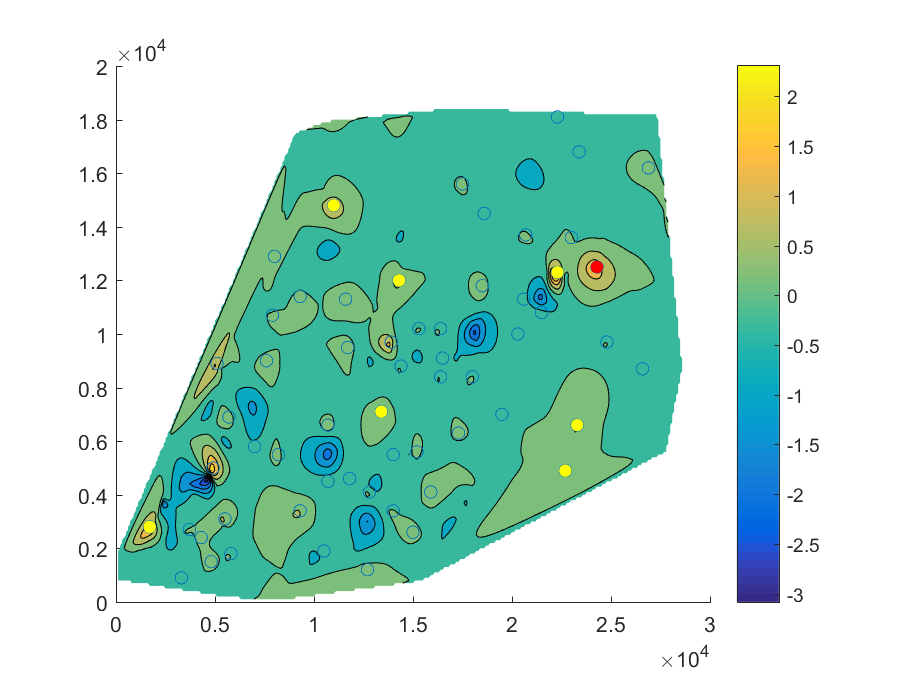
\includegraphics{pictures/polluted-source.eps}
    \caption{污染源分布图}
    \label{fig:polluted-source}
\end{figure}
图中用黄色和红色点标出的即为污染源,其中红色点表示污染最为严重的点。
\section{城市未来地质环境预测}
在这样的假设下,我们要预测未来的城市地质环境的变化。




\part{模型的完善}
土壤中重金属的来源是多途径的,首先是成土母质本身含有重金属,不同的母质、成土过程所形成的土壤含有重金属量差异很大。
此外,人类工农业生产活动,也造成重金属对大气、水体和土壤的污染,而大气和水体中的重金属又会反过来对土壤的污染造成影响。
在前面的建模过程中,我们仅仅只考虑了土壤和地势对于重金属传播的影响,而没有考虑水体以及空气的因素,












\end{document}